%! Author = Wiktor Rostkowski, Mateusz Budzisz
%! Date = 29/04/2024

\chapter{Podsumowanie}
\label{ch:podsumowanie}

\section{Napotkane wyzwania}
\label{sec:napotkane-wyzwania}

Największym wyzwaniem, z jakim zespół projektowy musiał się zmierzyć, był częściowy rozpad grupy, w wyniku którego zespół zmniejszył się o połowę.
To znaczące uszczuplenie liczby członków wpłynęło na zdolność zespołu do realizacji wszystkich zaplanowanych funkcjonalności.
W rezultacie projekt nie był w stanie w pełni zrealizować integracji z komunikacją miejską w Gdańsku, co było jedną z głównych funkcji przewidzianych w początkowym planie.
Ograniczenia te zmusiły zespół do priorytetyzacji innych elementów projektu oraz do poszukiwania alternatywnych rozwiązań, aby sprostać ograniczeniom zasobów i czasu.

Drugim największym wyzwaniem była implementacja kalendarza, który umożliwia planowanie zwiedzania w wybrane dni za pomocą funkcji przeciągnij i upuść.
Kalendarz ten uwzględnia godziny otwarcia atrakcji turystycznych oraz proponowany czas zwiedzania każdej atrakcji.
Algorytm kalendarza musi pilnować wszystkich tych ograniczeń, aby zaplanowany harmonogram był możliwy do zrealizowania w rzeczywistości.
Dodatkowo, możliwość zmiany czasu przeznaczonego na zwiedzanie przez użytkownika wprowadziła kolejny poziom skomplikowania, wymagając dynamicznej aktualizacji planu.
Ta funkcjonalność musiała również uwzględniać różne scenariusze i wyjątkowe przypadki, takie jak zmiany godzin otwarcia atrakcji w dni świąteczne czy nieprzewidziane zamknięcia, co dodatkowo komplikowało implementację.

\begin{figure}[H]
    \centering
    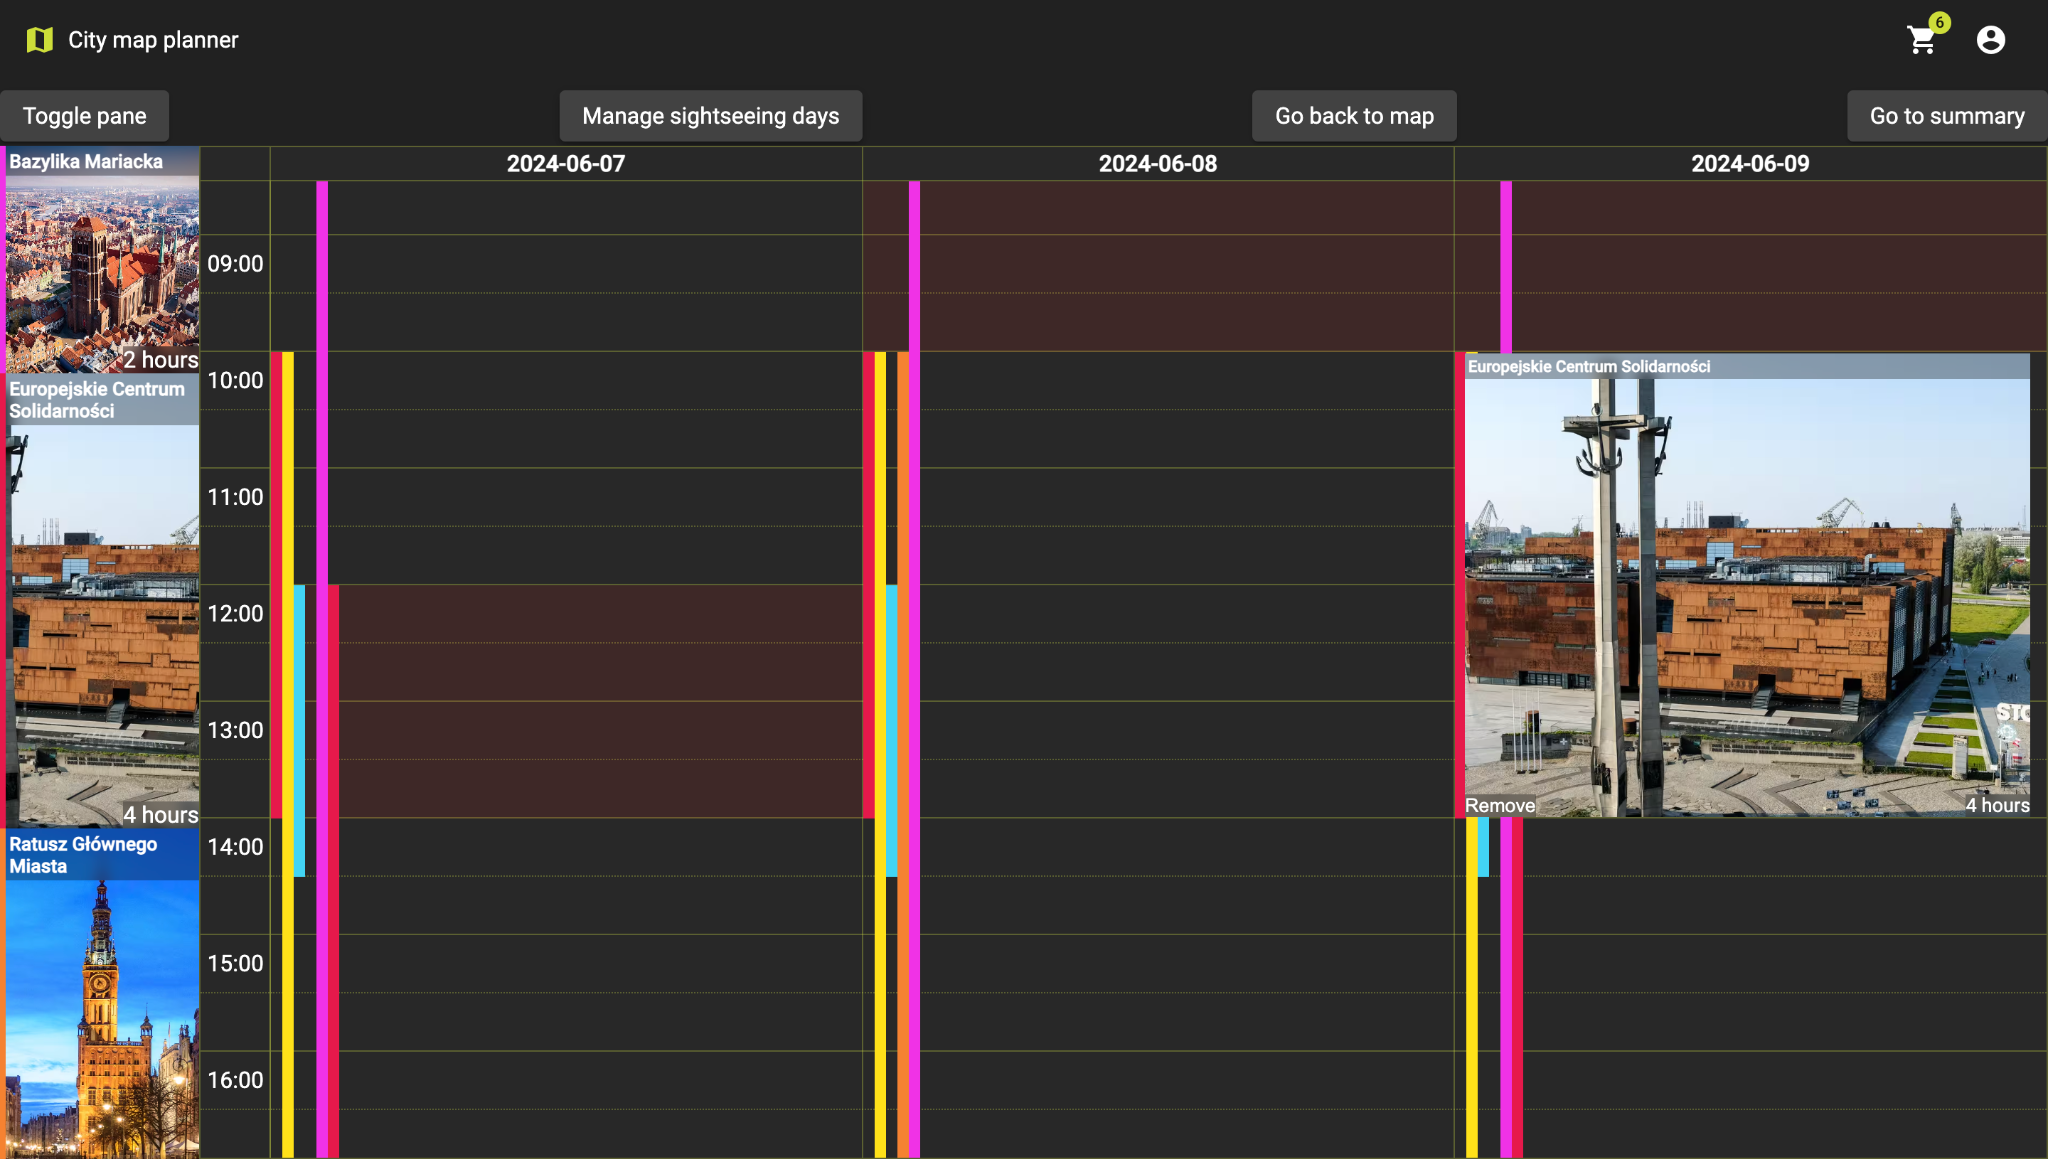
\includegraphics[width=1\textwidth]{attachments/t1}
    \caption{Screenshot przykładowego użycia kalendarza}
\end{figure}

Trzecim wyzwaniem, przed którym stanął zespół projektowy, była integracja menedżera punktów zainteresowania (POI) ze sztuczną inteligencją.
System co godzinę zapisuje snapshot stron internetowych atrakcji i porównuje je z wcześniejszymi wersjami w celu wykrycia zmian.
W przypadku wykrycia zmian, dane są przesyłane do modelu GPT-4 od OpenAI w celu ekstrakcji godzin otwarcia, co częściowo automatyzuje proces aktualizacji informacji.
Sztuczna inteligencja zwraca dane w formacie tabelki markdown z wartościami wymagającymi normalizacji.
Przetwarzanie tych zdenormalizowanych danych przed zapisaniem ich do finalnej tabeli w bazie danych stanowiło znaczące wyzwanie.
Ponadto konieczne było uwzględnienie i pokrycie wielu przypadków anomalii generowanych przez AI, co dodatkowo skomplikowało ten proces.
Wyzwanie to wymagało nie tylko solidnej wiedzy technicznej, ale także elastyczności w dostosowywaniu systemu do różnych formatów i źródeł danych.

\begin{figure}[H]
    \centering
    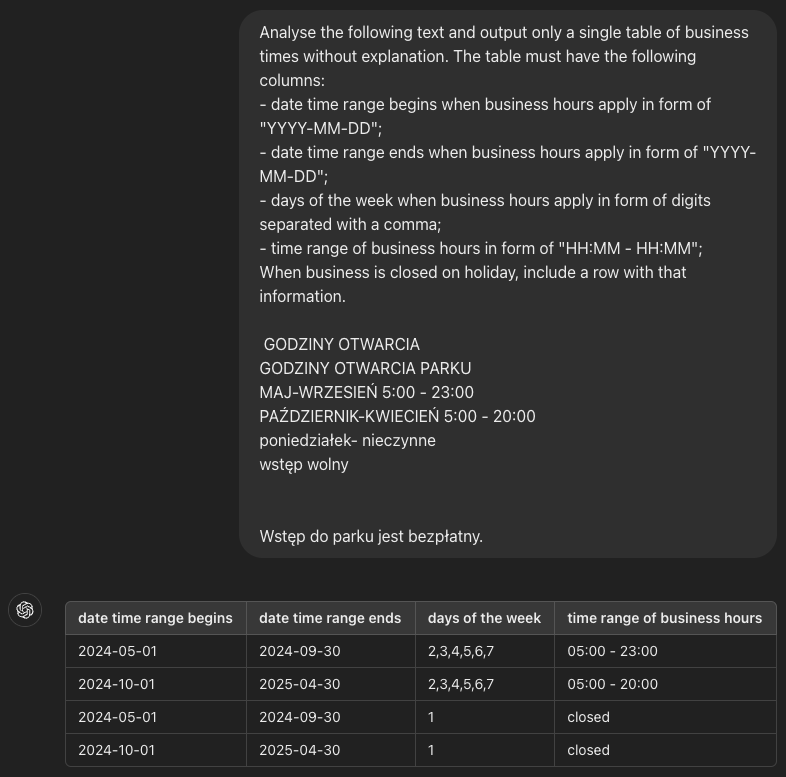
\includegraphics[width=1\textwidth]{attachments/t2}
    \caption{Przykład analizy AI}
\end{figure}

\section{Łączny nakład pracy}
\label{sec:laczny-naklad-pracy}

TODO

\section{Indywidualne wkłady pracy}
\label{sec:indywidualne-wklady-pracy}

\subsection{Mateusz Budzisz}
\label{subsec:mateusz-budzisz}

TODO

\subsection{Wiktor Rostkowski}
\label{subsec:wiktor-rostkowski}

TODO

\subsection{Damian Kreft}
\label{subsec:damian-kreft}

TODO

\subsection{Sebastian Kreft}
\label{subsec:sebastian-kreft}

TODO
